\documentclass[10pt]{article}
\usepackage[margin=0.7in]{geometry}\usepackage{amsmath,amssymb,tikz,hyperref}\setlength{\parindent}{0pt}\setlength{\parskip}{5pt}
\begin{document}
\textbf{Exact Scholten-to-weighted-model normalization}\hfill2026-10-31\\T-1130. Producer proof packet; independent source-fidelity review pending.
\section*{Checked model identity}
The source's fixed Gaussian constants give the quintic
\[F(t)=1+\frac{25}{3}t+\frac{299}{12}t^2+\frac{95}{3}t^3+\frac{187}{12}t^4+\frac52t^5.\]
The historical normalization helper uses $\alpha=5/2$, $\beta=-187/150$ and ordinate scale $\alpha^3=125/8$. Lean checks
\[F\left(\frac52x-\frac{187}{150}\right)=\left(\frac{125}{8}\right)^2N(x),\]
where
\begin{align*}
N(x)={}&x^5-\frac{12938}{28125}x^3+\frac{907312}{10546875}x^2\\
&+\frac{44207039}{1318359375}x-\frac{57913058672}{7415771484375}.
\end{align*}
The field hypotheses are $2,3,5\ne0$; source expansion also assumes $i^2=-1$. All denominator nonzeroness is explicit. These hypotheses cover the declared source primes $p>13$, without a new primality or cohort run.
\begin{center}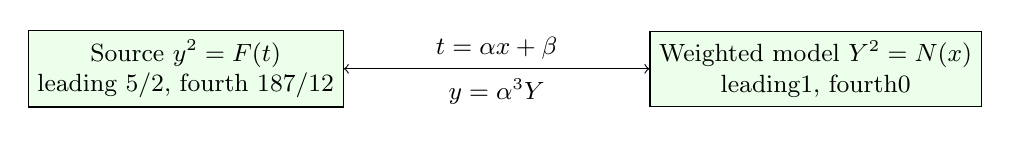
\begin{tikzpicture}[every node/.style={draw,align=center,font=\small}]
\node[fill=green!8] (a) at (0,0) {Source $y^2=F(t)$\\leading $5/2$, fourth $187/12$};
\node[fill=green!8] (b) at (8,0) {Weighted model $Y^2=N(x)$\\leading1, fourth0};
\draw[<->] (a)--node[above,draw=none] {$t=\alpha x+\beta$} node[below,draw=none] {$y=\alpha^3Y$}(b);
\end{tikzpicture}\end{center}
\section*{Formal scope}
Twelve main declarations establish source expansion, normalization, both coordinate round trips, curve-equation transport, evaluation in the existing \texttt{WeightedDoubling.curve} definition, and coefficients4/5 equal to0/1. Its parameter order is $(a_0,a_1,a_2,a_3)$.

Eight fixed controls check $F(0)=1$, $F(-1/2)=0$, coordinate values, wrong ordinate scaling, round trip and the helper's shift/scale. The $(t,y)=(3,7)$ fixture tests coordinate arithmetic; it is not asserted to lie on the curve. All20 declarations receive separate axiom readback. Fraction-pair polynomial expansion provides an additional producer cross-check, not independent review.
\section*{Connection to existing geometry}
The weighted-Proj and infinity-stalk modules already establish geometric properties of their model. Their Pic0Bridge explicitly does not construct a Picard group or a global class equality. This packet identifies the source's affine equation with that formula model. Global projective extension, squarefreeness transport, the literal Mumford substitution loops and Picard transport are next bindings; the affine identities do not silently supply them.
\section*{Evidence and sources}
Attempt1 failed on power rewriting/tactic sequencing; attempt2 passed. Successful inputs remain bound; linter warnings and the failure are retained. Source references: \texttt{three\_leads.rs}, lines1094--1171; historical \texttt{genus2\_model\_gate.rs}, lines14--56 and75--88. Primary documentation: \href{https://leanprover-community.github.io/mathlib4_docs/Mathlib/Algebra/Polynomial/Eval/Defs.html}{Mathlib polynomial evaluation and composition}. No novelty claim.

No scientific execution, timing or cost ratio; expired campaign limits unchanged. No independent binary/kernel rechecker or independent source-fidelity review is claimed. Full proof sources, raw receipts, coefficient JSON and source/custody hashes accompany this report.
\end{document}
